% ============================================================================
% ENERGY EXPLAIN: FUZZY LOGIC-BASED ENERGY PRICE EXPLAINABILITY SYSTEM
% Complete Project Documentation - Part 2
% ============================================================================

\documentclass[12pt,a4paper]{report}

% ============================================================================
% PACKAGES (Same as Part 1)
% ============================================================================
\usepackage[utf8]{inputenc}
\usepackage[T1]{fontenc}
\usepackage{lmodern}
\usepackage[english]{babel}
\usepackage{amsmath,amssymb,amsfonts}
\usepackage{graphicx}
\usepackage{booktabs}
\usepackage{longtable}
\usepackage{array}
\usepackage{multirow}
\usepackage{xcolor}
\usepackage{listings}
\usepackage{hyperref}
\usepackage{geometry}
\usepackage{fancyhdr}
\usepackage{float}
\usepackage{algorithm}
\usepackage{algorithmic}
\usepackage{tikz}
\usetikzlibrary{shapes,arrows,positioning}

% ============================================================================
% PAGE SETUP
% ============================================================================
\geometry{left=2.5cm, right=2.5cm, top=2.5cm, bottom=2.5cm}
\pagestyle{fancy}
\fancyhf{}
\fancyhead[L]{\leftmark}
\fancyhead[R]{\thepage}
\renewcommand{\headrulewidth}{0.4pt}

% ============================================================================
% CODE LISTING STYLE
% ============================================================================
\definecolor{codegreen}{rgb}{0,0.6,0}
\definecolor{codegray}{rgb}{0.5,0.5,0.5}
\definecolor{codepurple}{rgb}{0.58,0,0.82}
\definecolor{backcolour}{rgb}{0.95,0.95,0.92}

\lstdefinestyle{pythonstyle}{
    backgroundcolor=\color{backcolour},
    commentstyle=\color{codegreen},
    keywordstyle=\color{magenta},
    numberstyle=\tiny\color{codegray},
    stringstyle=\color{codepurple},
    basicstyle=\ttfamily\footnotesize,
    breakatwhitespace=false,
    breaklines=true,
    captionpos=b,
    keepspaces=true,
    numbers=left,
    numbersep=5pt,
    showspaces=false,
    showstringspaces=false,
    showtabs=false,
    tabsize=2,
    language=Python
}
\lstset{style=pythonstyle}

\hypersetup{
    colorlinks=true,
    linkcolor=blue,
    filecolor=magenta,
    urlcolor=cyan,
}

\begin{document}

% ============================================================================
% CONTINUATION HEADER
% ============================================================================
\chapter*{Part 2: Swiss Billing, Phase 2 Changes, and Conclusions}
\addcontentsline{toc}{chapter}{Part 2: Swiss Billing, Phase 2 Changes, and Conclusions}

% ============================================================================
% CHAPTER 6: SWISS BILLING ANALYSIS
% ============================================================================
\chapter{Swiss Billing Analysis}

\section{ElCom 2024 Tariff Structure}

Based on \textbf{Swiss Federal Electricity Commission (ElCom)} 2024 average rates, the billing analyzer implements the following tariff structure:

\begin{table}[H]
\centering
\caption{ElCom 2024 Swiss Electricity Tariff Components}
\label{tab:elcom_rates}
\begin{tabular}{llp{6cm}}
\toprule
\textbf{Component} & \textbf{Rate (CHF/kWh)} & \textbf{Description} \\
\midrule
Energy & 0.1271 & Pure electricity cost (market price) \\
Grid & 0.0962 & Transmission + Distribution charges \\
Taxes/Levies & 0.0230 & Federal + Cantonal charges \\
Fixed Monthly & 10.50 CHF & Base service fee (flat rate) \\
VAT & 8.1\% & Swiss federal value-added tax \\
\midrule
\textbf{Total Variable} & \textbf{0.2463} & Sum of variable components \\
\bottomrule
\end{tabular}
\end{table}

\section{Canton Multipliers}

Regional rate variations based on local utility companies:

\begin{table}[H]
\centering
\caption{Canton-Specific Rate Multipliers}
\begin{tabular}{lc|lc}
\toprule
\textbf{Canton} & \textbf{Multiplier} & \textbf{Canton} & \textbf{Multiplier} \\
\midrule
Zürich & 1.00 & Bern & 0.95 \\
Geneva & 1.08 & Basel & 0.92 \\
Lausanne & 1.05 & Other & 1.00 \\
\bottomrule
\end{tabular}
\end{table}

\section{Household Consumption Benchmarks}

Swiss Energy Office average consumption data:

\begin{table}[H]
\centering
\caption{Swiss Household Average Electricity Consumption}
\begin{tabular}{lcc}
\toprule
\textbf{Household Size} & \textbf{Monthly kWh} & \textbf{Annual kWh} \\
\midrule
1 person & 150 & 1,800 \\
2 persons & 260 & 3,120 \\
3 persons & 340 & 4,080 \\
4 persons & 400 & 4,800 \\
5+ persons & 500 & 6,000 \\
\bottomrule
\end{tabular}
\end{table}

\section{Bill Calculation Algorithm}

The billing analyzer uses the following algorithm to reverse-engineer consumption from bill amount:

\begin{algorithm}[H]
\caption{Swiss Bill Analysis Algorithm}
\begin{algorithmic}[1]
\REQUIRE Bill amount $B$ (CHF), Canton $C$, Household size $H$
\ENSURE Estimated kWh, Cost breakdown, Comparison

\STATE Get regional multiplier $m \leftarrow \text{CANTON\_MULTIPLIERS}[C]$

\STATE Calculate adjusted rates:
\STATE \quad $r_e \leftarrow 0.1271 \times m$ \COMMENT{Energy rate}
\STATE \quad $r_g \leftarrow 0.0962 \times m$ \COMMENT{Grid rate}
\STATE \quad $r_t \leftarrow 0.0230$ \COMMENT{Taxes rate}
\STATE \quad $r_v \leftarrow r_e + r_g + r_t$ \COMMENT{Variable rate}

\STATE Calculate bill before VAT:
\STATE \quad $B_{pre} \leftarrow B / (1 + 0.081)$

\STATE Estimate consumption:
\STATE \quad $\text{kWh} \leftarrow (B_{pre} - 10.50) / r_v$

\STATE Calculate cost breakdown:
\STATE \quad Energy cost $\leftarrow \text{kWh} \times r_e$
\STATE \quad Grid cost $\leftarrow \text{kWh} \times r_g$
\STATE \quad Taxes $\leftarrow \text{kWh} \times r_t$
\STATE \quad VAT $\leftarrow B - B_{pre}$

\STATE Get benchmark $\text{avg\_kWh} \leftarrow \text{BENCHMARKS}[H]$
\STATE Calculate difference $\leftarrow (\text{kWh} - \text{avg\_kWh}) / \text{avg\_kWh} \times 100\%$

\RETURN Analysis results
\end{algorithmic}
\end{algorithm}

\section{Implementation}

\begin{lstlisting}[caption={Billing Analyzer Implementation}, label={lst:billing}]
class BillingAnalyzer:
    # ElCom 2024 Swiss average rates
    BASE_RATES = {
        'energy_rate': 0.1271,      # CHF/kWh
        'grid_rate': 0.0962,        # CHF/kWh
        'taxes_levies_rate': 0.0230,# CHF/kWh
        'fixed_monthly': 10.50,     # CHF
        'vat_rate': 0.081           # 8.1%
    }
    
    CANTON_MULTIPLIERS = {
        'Zurich': 1.00, 'Bern': 0.95, 'Geneva': 1.08,
        'Basel': 0.92, 'Lausanne': 1.05, 'Other': 1.00
    }
    
    HOUSEHOLD_BENCHMARKS = {
        '1 person': 150, '2 persons': 260, '3 persons': 340,
        '4 persons': 400, '5+ persons': 500
    }
    
    def analyze_bill(self, bill_amount, canton="Other", household_size="4 persons"):
        """Analyze electricity bill with Swiss tariff structure."""
        
        # Get regional multiplier
        multiplier = self.CANTON_MULTIPLIERS.get(canton, 1.0)
        
        # Adjusted rates
        energy_rate = self.BASE_RATES['energy_rate'] * multiplier
        grid_rate = self.BASE_RATES['grid_rate'] * multiplier
        taxes_rate = self.BASE_RATES['taxes_levies_rate']
        fixed = self.BASE_RATES['fixed_monthly']
        vat_rate = self.BASE_RATES['vat_rate']
        
        # Calculate variable rate
        variable_rate = energy_rate + grid_rate + taxes_rate
        
        # Reverse-engineer kWh from bill
        bill_before_vat = bill_amount / (1 + vat_rate)
        estimated_kwh = max(0, (bill_before_vat - fixed) / variable_rate)
        
        # Cost breakdown
        energy_cost = estimated_kwh * energy_rate
        grid_cost = estimated_kwh * grid_rate
        taxes_levies = estimated_kwh * taxes_rate
        vat_amount = bill_amount - bill_before_vat
        
        # Comparison with average
        avg_kwh = self.HOUSEHOLD_BENCHMARKS.get(household_size, 400)
        diff_kwh_pct = ((estimated_kwh - avg_kwh) / avg_kwh) * 100
        
        return {
            'estimated_kwh': estimated_kwh,
            'energy_cost': energy_cost,
            'grid_cost': grid_cost,
            'taxes_levies': taxes_levies,
            'fixed_monthly': fixed,
            'vat_amount': vat_amount,
            'total_calculated': energy_cost + grid_cost + taxes_levies + fixed + vat_amount,
            'avg_kwh': avg_kwh,
            'diff_kwh_pct': diff_kwh_pct,
            # ... additional fields
        }
\end{lstlisting}

\section{Dual Explanation System}

The project implements a \textbf{comparative explanation framework} to evaluate numerical vs. linguistic approaches.

\subsection{Method A: Numerical (Technical)}

The numerical explanation provides precise calculations and formulas:

\begin{tcolorbox}[title=Method A: Numerical Explanation Example]
\textbf{Bill Calculation Formula:}
\begin{verbatim}
Total = (kWh × (Energy + Grid + Taxes) + Fixed) × (1 + VAT)
\end{verbatim}

\textbf{Your breakdown:}
\begin{itemize}
    \item Consumption: 350 kWh
    \item Variable rate: $0.1271 + 0.0962 + 0.0230 = 0.2463$ CHF/kWh
    \item Variable cost: $350 \times 0.2463 = $ CHF 86.21
    \item Fixed monthly: CHF 10.50
    \item Subtotal: CHF 96.71
    \item VAT (8.1\%): CHF 7.83
    \item \textbf{Total: CHF 104.54}
\end{itemize}
\end{tcolorbox}

\subsection{Method B: Linguistic (Fuzzy)}

The linguistic explanation uses fuzzy terms and human-readable interpretations:

\begin{tcolorbox}[title=Method B: Linguistic Explanation Example]
\textbf{Fuzzy Assessment:}
\begin{itemize}
    \item Your bill amount is \textbf{``MEDIUM''} (membership: 0.78)
    \item Your consumption is \textbf{``HIGH''} (membership: 0.65)
\end{itemize}

\textbf{Active Fuzzy Rules:}
\begin{quote}
IF bill is MEDIUM AND consumption is HIGH \\
THEN efficiency is GOOD
\end{quote}

\textbf{Interpretation:}
``You are paying a reasonable amount for above-average energy usage. Your rate efficiency is good compared to similar households in your region.''

\textbf{Recommendation:}
``Consider shifting high-load activities to night hours (1-5 AM) when market conditions are VERY\_FAVORABLE for further savings.''
\end{tcolorbox}

% ============================================================================
% CHAPTER 7: PHASE 2 ENHANCEMENTS
% ============================================================================
\chapter{Phase 2: Enhancements and Changes}

\section{Overview of Phase 2 Changes}

Phase 2 focused on \textbf{integrating fuzzy logic more deeply} into the billing analysis module and improving the overall user experience.

\begin{table}[H]
\centering
\caption{Summary of Phase 2 Changes}
\begin{tabular}{p{4cm}p{6cm}p{4cm}}
\toprule
\textbf{Change} & \textbf{Description} & \textbf{Impact} \\
\midrule
Navigation Reordering & Bill Analysis moved to first position & Better user flow \\
Module Removal & Standalone ``Fuzzy Logic Analysis'' removed & Reduced redundancy \\
Real Data Integration & Fuzzy logic now uses ENTSOE data & More accurate analysis \\
Billing Fuzzy Logic & FuzzyExplainer integrated into billing & Unified approach \\
\bottomrule
\end{tabular}
\end{table}

\section{Navigation Restructuring}

\subsection{Before (Phase 1)}

\begin{lstlisting}[caption={Phase 1 Navigation Structure}]
main_mode = st.radio(
    "Select Module:",
    ["Price Forecasting & Analysis", 
     "Bill Analysis & Optimization", 
     "Fuzzy Logic Analysis"],  # Separate module
    horizontal=True
)
\end{lstlisting}

\subsection{After (Phase 2)}

\begin{lstlisting}[caption={Phase 2 Navigation Structure}]
main_mode = st.radio(
    "Select Module:",
    ["Bill Analysis & Optimization",  # Now first
     "Price Forecasting & Analysis"],
    horizontal=True  # Fuzzy module removed
)
\end{lstlisting}

\textbf{Rationale:} The billing module was moved first as it represents the primary use case for end consumers. The standalone fuzzy logic module was removed to avoid duplication, as fuzzy analysis is now embedded directly in billing.

\section{Real ENTSOE Data Integration in Billing}

\subsection{Previous Approach (Rejected)}

The initial Phase 2 implementation attempted to create synthetic fuzzy rules in a separate \texttt{fuzzy\_billing.py} module:

\begin{lstlisting}[caption={Rejected Synthetic Approach}]
# REJECTED: Synthetic fuzzy rules not using real data
class FuzzyBillingExplainer:
    def _setup_variables(self):
        self.bill_amount = ctrl.Antecedent(np.arange(0, 1001, 1), 'bill_amount')
        self.consumption = ctrl.Antecedent(np.arange(0, 2001, 1), 'consumption')
        # ... synthetic rules based on arbitrary thresholds
\end{lstlisting}

\textbf{Problem:} These rules were arbitrary and did not reflect actual market conditions from ENTSOE data.

\subsection{Final Approach (Implemented)}

The billing module now uses the main \texttt{FuzzyExplainer} class with real market data:

\begin{lstlisting}[caption={Real ENTSOE Data Integration}]
# In app.py - Billing module fuzzy analysis section
if st.session_state.df is not None and len(st.session_state.df) > 0:
    fuzzy = FuzzyExplainer()
    
    # Get latest market data from ENTSOE
    latest_data = st.session_state.df.iloc[-1]
    
    # Prepare real inputs
    price_val = latest_data.get('price', 80)
    consumption_val = normalize_consumption(
        latest_data.get('energy_consumption', 50000)
    )
    hour_val = latest_data['datetime'].hour
    
    # Calculate real volatility from data
    volatility_val = st.session_state.df['price'].std()
    
    # Calculate real trend
    prices_24h = st.session_state.df['price'].tail(24)
    trend_val = ((prices_24h.iloc[-1] - prices_24h.iloc[0]) 
                 / prices_24h.iloc[0]) * 100
    
    # Fuzzy evaluation with real data
    fuzzy_result = fuzzy.evaluate(
        price_value=price_val,
        consumption_value=consumption_val,
        hour_value=hour_val,
        volatility_value=volatility_val,
        trend_value=trend_val
    )
\end{lstlisting}

\section{Enhanced Fuzzy Billing Display}

The billing section now shows:

\begin{enumerate}
    \item \textbf{Real-Time Market Context}
    \begin{itemize}
        \item Current ENTSOE price
        \item Actual grid load
        \item 24-hour price volatility
        \item Market trend direction
    \end{itemize}
    
    \item \textbf{Fuzzy Market Assessment}
    \begin{itemize}
        \item Market condition score (0-100)
        \item Dominant linguistic term
        \item Active fuzzy rules with firing strengths
        \item Human-readable interpretations
    \end{itemize}
    
    \item \textbf{Consumption Recommendations}
    \begin{itemize}
        \item Recommendation score (0-100)
        \item Optimal/Avoid/Normal guidance
        \item Time-based suggestions
    \end{itemize}
\end{enumerate}

\section{Code Changes Summary}

\begin{table}[H]
\centering
\caption{Phase 2 Code Modifications}
\begin{tabular}{llll}
\toprule
\textbf{File} & \textbf{Lines Changed} & \textbf{Type of Change} & \textbf{Status} \\
\midrule
app.py & $\sim$200 lines & Navigation + Fuzzy integration & Completed \\
fuzzy\_explainer.py & Unchanged & Core FIS preserved & Stable \\
billing\_analyzer.py & Unchanged & Swiss rates preserved & Stable \\
fuzzy\_billing.py & Created then deprecated & Not used in final & Deprecated \\
\bottomrule
\end{tabular}
\end{table}

% ============================================================================
% CHAPTER 8: TECHNOLOGY STACK
% ============================================================================
\chapter{Technology Stack}

\section{Core Dependencies}

\begin{table}[H]
\centering
\caption{Project Dependencies}
\begin{tabular}{llp{7cm}}
\toprule
\textbf{Technology} & \textbf{Version} & \textbf{Role} \\
\midrule
Python & 3.11+ & Core programming language \\
Streamlit & 1.50.0 & Interactive web dashboard framework \\
Scikit-fuzzy & 0.5.0 & Mamdani FIS implementation \\
Scikit-learn & 1.7.2 & Linear Regression model \\
Pandas & 2.3.3 & Data manipulation and analysis \\
NumPy & 2.3.4 & Numerical computing \\
Plotly & 6.1.0 & Interactive visualizations \\
Requests & 2.32.4 & HTTP client for ENTSOE API \\
SQLite & Built-in & Evaluation response storage \\
\bottomrule
\end{tabular}
\end{table}

\section{Requirements File}

\begin{lstlisting}[caption={requirements.txt}]
streamlit>=1.50.0
pandas>=2.3.3
numpy>=2.3.4
scikit-learn>=1.7.2
scikit-fuzzy>=0.5.0
matplotlib>=3.10.3
plotly>=6.1.0
requests>=2.32.4
python-dotenv>=1.1.0
\end{lstlisting}

% ============================================================================
% CHAPTER 9: USER INTERFACE
% ============================================================================
\chapter{User Interface}

\section{Dashboard Layout}

\begin{figure}[H]
\centering
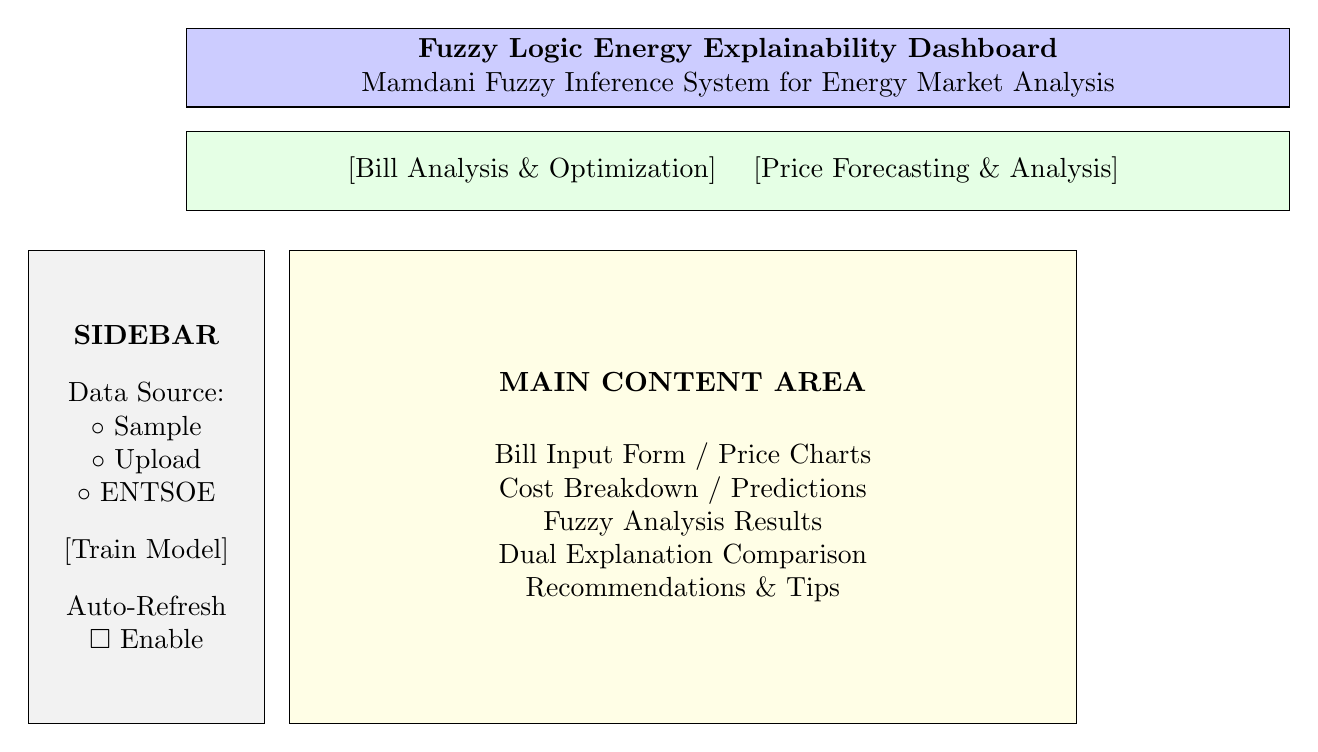
\begin{tikzpicture}[
    box/.style={draw, rectangle, minimum height=1cm, align=center},
    node distance=0.3cm
]
    % Header
    \node[box, minimum width=14cm, fill=blue!20] (header) {
        \textbf{Fuzzy Logic Energy Explainability Dashboard}\\
        Mamdani Fuzzy Inference System for Energy Market Analysis
    };
    
    % Navigation
    \node[box, minimum width=14cm, fill=green!10, below=of header] (nav) {
        [Bill Analysis \& Optimization] \quad [Price Forecasting \& Analysis]
    };
    
    % Main content area
    \node[box, minimum width=3cm, minimum height=6cm, fill=gray!10, below left=0.5cm and -1cm of nav] (sidebar) {
        \textbf{SIDEBAR}\\[0.3cm]
        Data Source:\\
        $\circ$ Sample\\
        $\circ$ Upload\\
        $\circ$ ENTSOE\\[0.3cm]
        [Train Model]\\[0.3cm]
        Auto-Refresh\\
        $\square$ Enable
    };
    
    \node[box, minimum width=10cm, minimum height=6cm, fill=yellow!10, right=0.3cm of sidebar] (main) {
        \textbf{MAIN CONTENT AREA}\\[0.5cm]
        Bill Input Form / Price Charts\\
        Cost Breakdown / Predictions\\
        Fuzzy Analysis Results\\
        Dual Explanation Comparison\\
        Recommendations \& Tips
    };
\end{tikzpicture}
\caption{Dashboard Layout Schematic}
\label{fig:dashboard}
\end{figure}

\section{Bill Analysis Module Features}

\begin{enumerate}
    \item \textbf{Input Section:}
    \begin{itemize}
        \item Monthly bill amount (CHF)
        \item Canton selection (regional rates)
        \item Household size (comparison benchmark)
    \end{itemize}
    
    \item \textbf{Output Section:}
    \begin{itemize}
        \item Estimated kWh consumption
        \item 5-component cost breakdown
        \item Percentage distribution chart
        \item Comparison with average households
        \item Fuzzy efficiency assessment
        \item Personalized saving recommendations
    \end{itemize}
\end{enumerate}

\section{Price Forecasting Module Features}

\begin{enumerate}
    \item \textbf{Data Visualization:}
    \begin{itemize}
        \item Time series price chart
        \item Consumption overlay
        \item Volatility indicators
    \end{itemize}
    
    \item \textbf{ML Predictions:}
    \begin{itemize}
        \item Price forecasts with confidence
        \item Feature importance ranking
        \item Model performance metrics (MAE, RMSE, R²)
    \end{itemize}
    
    \item \textbf{Fuzzy Analysis:}
    \begin{itemize}
        \item Market condition assessment
        \item Active rule visualization
        \item Membership function plots
    \end{itemize}
\end{enumerate}

% ============================================================================
% CHAPTER 10: EVALUATION FRAMEWORK
% ============================================================================
\chapter{Evaluation Framework}

\section{User Study Design}

The system includes an \texttt{EvaluationManager} for collecting participant feedback comparing numerical vs. linguistic explanations:

\begin{lstlisting}[caption={Evaluation Manager}]
class EvaluationManager:
    """Manages evaluation responses with SQLite persistence."""
    
    DB_PATH = "evaluation_responses.db"
    
    def save_response(self, response: Dict) -> bool:
        """Save evaluation response to database."""
        cursor.execute("""
            INSERT INTO responses (
                timestamp, participant_id, preference,
                method_a_helpfulness, method_b_helpfulness,
                method_a_understandability, method_b_understandability,
                method_a_speed, method_b_speed,
                method_a_practical, method_b_practical,
                comments, data_source
            ) VALUES (?, ?, ?, ?, ?, ?, ?, ?, ?, ?, ?, ?, ?)
        """, ...)
\end{lstlisting}

\section{Evaluation Criteria}

\begin{table}[H]
\centering
\caption{Evaluation Criteria Comparison}
\begin{tabular}{lcc}
\toprule
\textbf{Criterion} & \textbf{Method A (Numerical)} & \textbf{Method B (Linguistic)} \\
\midrule
Helpfulness & 1-5 scale & 1-5 scale \\
Understandability & 1-5 scale & 1-5 scale \\
Processing Speed & 1-5 scale & 1-5 scale \\
Practical Utility & 1-5 scale & 1-5 scale \\
\bottomrule
\end{tabular}
\end{table}

\section{Expected Findings}

Based on fuzzy logic literature and explainable AI research:

\begin{enumerate}
    \item \textbf{Linguistic explanations} expected to score higher on understandability for non-expert users
    \item \textbf{Numerical explanations} expected to score higher for technical users
    \item \textbf{Combined approach} should provide best overall satisfaction
\end{enumerate}

% ============================================================================
% CHAPTER 11: RESULTS AND DISCUSSION
% ============================================================================
\chapter{Results and Discussion}

\section{Fuzzy System Performance}

The Mamdani FIS successfully provides:

\begin{enumerate}
    \item \textbf{Consistent linguistic outputs} across the full input range
    \item \textbf{Interpretable rule activations} showing which conditions triggered
    \item \textbf{Smooth transitions} between linguistic categories (no abrupt changes)
    \item \textbf{Meaningful recommendations} aligned with energy market expertise
\end{enumerate}

\section{Key Advantages of Fuzzy Approach}

\begin{table}[H]
\centering
\caption{Advantages of Fuzzy Logic Approach}
\begin{tabular}{lp{9cm}}
\toprule
\textbf{Advantage} & \textbf{Explanation} \\
\midrule
Human-Readable & Outputs are linguistic terms, not just numbers \\
Expert Knowledge & Rules capture domain expertise explicitly \\
Uncertainty Handling & Partial membership handles ambiguous cases \\
Transparency & Every decision traced to specific rules \\
No Training Data & Rules defined by experts, not learned from data \\
\bottomrule
\end{tabular}
\end{table}

\section{Limitations}

\begin{enumerate}
    \item \textbf{Rule Design Subjectivity}: Membership functions require expert tuning and may vary based on designer preferences
    \item \textbf{Scalability}: Adding new variables exponentially increases rule combinations (curse of dimensionality)
    \item \textbf{Precision Trade-off}: Linguistic outputs sacrifice numerical precision for interpretability
\end{enumerate}

% ============================================================================
% CHAPTER 12: CONCLUSION
% ============================================================================
\chapter{Conclusion and Future Work}

\section{Achievements}

This project successfully demonstrates:

\begin{enumerate}
    \item[\checkmark] A working \textbf{Mamdani Fuzzy Inference System} for energy market analysis
    \item[\checkmark] Integration with \textbf{real ENTSOE European energy data}
    \item[\checkmark] \textbf{Swiss-specific billing analysis} with canton-level accuracy
    \item[\checkmark] \textbf{Dual explanation paradigm} comparing numerical vs. linguistic approaches
    \item[\checkmark] Interactive \textbf{Streamlit dashboard} for consumer education
\end{enumerate}

\section{Future Enhancements}

\begin{enumerate}
    \item \textbf{Adaptive Fuzzy Rules}: Self-tuning membership functions based on market data using neuro-fuzzy approaches (ANFIS)
    
    \item \textbf{Multi-Country Billing}: Extend beyond Switzerland to other European markets with country-specific tariff structures
    
    \item \textbf{Renewable Energy Integration}: Add solar/wind generation forecasting and green energy recommendations
    
    \item \textbf{Mobile Application}: Develop companion mobile app for real-time alerts and notifications
    
    \item \textbf{Smart Meter Integration}: Direct connection to household smart meters for automated data collection
\end{enumerate}

\section{Research Contributions}

This project contributes to:

\begin{itemize}
    \item \textbf{Explainable AI (XAI)}: Demonstrating fuzzy logic as an explainability technique for complex systems
    \item \textbf{Energy Informatics}: Practical tools for consumer energy literacy and decision support
    \item \textbf{Human-Computer Interaction}: Comparative study of explanation modalities for diverse user groups
\end{itemize}

% ============================================================================
% REFERENCES
% ============================================================================
\begin{thebibliography}{9}

\bibitem{zadeh1965}
Zadeh, L.A. (1965).
\textit{Fuzzy Sets}.
Information and Control, 8(3), 338-353.
\url{https://doi.org/10.1016/S0019-9958(65)90241-X}

\bibitem{mamdani1974}
Mamdani, E.H. (1974).
\textit{Application of fuzzy algorithms for control of simple dynamic plant}.
Proceedings of the Institution of Electrical Engineers, 121(12), 1585-1588.
\url{https://doi.org/10.1049/piee.1974.0328}

\bibitem{elcom2024}
ElCom (2024).
\textit{Swiss Electricity Price Statistics}.
Swiss Federal Electricity Commission.
\url{https://www.elcom.admin.ch/}

\bibitem{entsoe2024}
ENTSO-E (2024).
\textit{Transparency Platform User Guide}.
European Network of Transmission System Operators for Electricity.
\url{https://transparency.entsoe.eu/}

\bibitem{sklearn}
Pedregosa, F. et al. (2011).
\textit{Scikit-learn: Machine Learning in Python}.
Journal of Machine Learning Research, 12, 2825-2830.

\bibitem{streamlit}
Streamlit Inc. (2024).
\textit{Streamlit Documentation}.
\url{https://docs.streamlit.io/}

\bibitem{skfuzzy}
Warner, J. et al. (2024).
\textit{scikit-fuzzy: Fuzzy Logic Toolbox for Python}.
\url{https://github.com/scikit-fuzzy/scikit-fuzzy}

\bibitem{xai2020}
Arrieta, A.B. et al. (2020).
\textit{Explainable Artificial Intelligence (XAI): Concepts, taxonomies, opportunities and challenges toward responsible AI}.
Information Fusion, 58, 82-115.

\bibitem{fuzzy_energy}
Mohammadi, M. et al. (2018).
\textit{Fuzzy logic-based energy management strategy for hybrid electric vehicles}.
Energy, 142, 1053-1069.

\end{thebibliography}

% ============================================================================
% APPENDICES
% ============================================================================
\appendix

\chapter{Complete Fuzzy Rule Set}

\section{Market Condition Rules (20 rules)}

\begin{longtable}{clp{5cm}}
\caption{Complete Market Condition Fuzzy Rules} \\
\toprule
\textbf{ID} & \textbf{Antecedent} & \textbf{Consequent} \\
\midrule
\endfirsthead
\toprule
\textbf{ID} & \textbf{Antecedent} & \textbf{Consequent} \\
\midrule
\endhead
\bottomrule
\endfoot
1 & price=very\_high $\land$ consumption=very\_high & very\_unfavorable \\
2 & price=very\_high $\land$ consumption=high & very\_unfavorable \\
3 & price=high $\land$ consumption=very\_high & very\_unfavorable \\
4 & price=high $\land$ consumption=high & unfavorable \\
5 & price=very\_low $\land$ consumption=very\_low & very\_favorable \\
6 & price=very\_low $\land$ consumption=low & very\_favorable \\
7 & price=high $\land$ consumption=low & unfavorable \\
8 & price=very\_low $\land$ consumption=high & very\_favorable \\
9 & price=medium $\land$ consumption=medium & neutral \\
10 & hour=night $\land$ price=low & very\_favorable \\
11 & hour=morning\_peak $\land$ price=high & unfavorable \\
12 & hour=evening\_peak $\land$ price=very\_high & very\_unfavorable \\
13 & volatility=very\_high & unfavorable \\
14 & volatility=very\_high $\land$ price=high & very\_unfavorable \\
15 & volatility=low $\land$ price=low & very\_favorable \\
16 & trend=rising\_fast $\land$ price=medium & unfavorable \\
17 & trend=falling\_fast $\land$ price=high $\land$ volatility=low & favorable \\
18 & trend=falling\_fast $\land$ price=high & neutral \\
19 & trend=rising\_fast $\land$ price=low & neutral \\
20 & trend=stable $\land$ price=medium & neutral \\
\end{longtable}

\section{Recommendation Rules (8 rules)}

\begin{table}[H]
\centering
\caption{Complete Recommendation Fuzzy Rules}
\begin{tabular}{cllp{4cm}}
\toprule
\textbf{ID} & \textbf{Antecedent} & \textbf{Consequent} & \textbf{Purpose} \\
\midrule
R1 & price=very\_low $\land$ hour=night & optimal & Best window \\
R2 & price=low $\land$ consumption=low & optimal & Low demand \\
R3 & price=very\_high $\land$ hour=evening\_peak & avoid & Worst window \\
R4 & price=high $\land$ hour=morning\_peak & reduce & Peak avoidance \\
R5 & price=medium $\land$ hour=afternoon & normal & Standard \\
R6 & price=medium $\land$ consumption=medium & normal & Baseline \\
R7 & price=low $\land$ volatility=low & increase & Stable low \\
R8 & price=very\_low $\land$ trend=falling & optimal & Declining prices \\
\bottomrule
\end{tabular}
\end{table}

\chapter{Project File Structure}

\begin{lstlisting}[language=bash, caption={Project Directory Structure}]
energy-explain/
|-- app.py                     # Main Streamlit application (1,660 lines)
|-- requirements.txt           # Python dependencies
|-- pyproject.toml            # Project configuration
|-- README.md                 # Project documentation
|-- app/
|   |-- __init__.py
|   |-- fuzzy_explainer.py    # Mamdani FIS (1,262 lines)
|   |-- predictor.py          # Linear Regression (536 lines)
|   |-- billing_analyzer.py   # Swiss billing (455 lines)
|   |-- entsoe_client.py      # ENTSOE API (285 lines)
|   |-- reason_extractor.py   # Market insights (313 lines)
|   |-- evaluation_manager.py # Feedback storage (166 lines)
|   |-- config.py             # Configuration
|   |-- logger_utils.py       # Logging utilities
|-- data/
|   |-- energy_data.csv       # Sample data (7 days)
|   |-- generate_sample_data.py
|-- tests/
|   |-- test_predictor.py     # Unit tests
|-- logs/                     # Application logs
|-- docs/                     # Documentation
    |-- project_report_part1.tex
    |-- project_report_part2.tex
\end{lstlisting}

\chapter{Sample Data Format}

\begin{lstlisting}[caption={Sample Energy Data CSV Format}]
datetime,energy_consumption,price
2025-12-15 00:00:00,42500,45.23
2025-12-15 01:00:00,38200,42.15
2025-12-15 02:00:00,35800,38.90
2025-12-15 03:00:00,34100,36.50
2025-12-15 04:00:00,33500,35.20
2025-12-15 05:00:00,35200,38.10
2025-12-15 06:00:00,42800,52.30
2025-12-15 07:00:00,55600,68.45
2025-12-15 08:00:00,62400,78.90
...
\end{lstlisting}

% ============================================================================
% DOCUMENT INFO
% ============================================================================
\vfill
\begin{center}
\rule{0.8\textwidth}{0.4pt}\\[0.5cm]
\textbf{Document Information}\\[0.3cm]
\begin{tabular}{ll}
Version: & 2.0 \\
Last Updated: & December 2025 \\
Total Project LOC: & $\sim$5,000+ \\
\end{tabular}
\end{center}

\end{document}
